\chapter{Биометрия радужки}

\section{Обзор методов биометрического распознавания}
\label{sec:beometric_methods_overview}

\textit{Биометрия (или биометрика)} - область знаний, изучающая методы и средства измерения и формализации персональных физических характеристик, поведенческих черт человека и их использование для идентификации или верификации человека.
\textit{Биометрической характеристикой человека (БХЧ)}) называются результаты измерения элемента фенотипа человека или поведенческой черты, в процессе сравнения которых с аналогичными, ранее зарегистрированными БХЧ (эталон, шаблон) реализуется процедура идентификации или верификации личности.

Биометрическая система представляет собой автоматизированную систему, решающую задачи идентификации или верификации личности и реализующую следующие операции~\cite{bmstu_biometrics}:

\begin{itemize}
	\setlength\itemsep{0.01em}
	\item[$\bullet$] регистрации выборки БХЧ от конкретного пользователя;
	\item[$\bullet$] формирование вектора биометрических данных из выборки БХЧ;
	\item[$\bullet$] формирование биометрического вектора признаков;
	\item[$\bullet$] сравнение биометрических векторов признаков с эталонами (шаблонами);
	\item[$\bullet$] принятие решения о соответствии сравниваемых БХЧ;
	\item[$\bullet$] формирование результата о достижении идентификации (верификации);
	\item[$\bullet$] принятие решения о повторении, окончании или видоизменении процесса идентификации (верификации).
\end{itemize}

Все БХЧ могут быть поделены на две группы: физиологические (статические) и поведенческие (динамические)~\cite{bmstu_biometrics}. Для каждой из груп насчитывается множество конкретных методов, наиболее распространенные из которых перечислены ниже:

\begin{enumerate}
	\setlength\itemsep{0.01em}
	\item Физиологические биометрические характеристики человека:
	\begin{enumerate}
		\item Видеообраз лица: овал, форма, размер отдельных деталей, геометрические параметры (расстояние между его определенными точками), узор подкожных кровеносных сосудов и др.;
		\item Структура радужной оболочки глаза;
		\item Структура кровеносных сосудов на сетчатке глаза;
		\item Особенности папиллярного узора одного или нескольких пальцев, ладони: параметры минуций (координаты, ориентация), параметры пространственно-частотного спектра и др.;
		\item Особенности папиллярного узора ладони;
		\item Особенности строения ладони: геометрия (ширина, длина, высота пальцев, расстояние между определенными точками), неровности складок кожи, рисунок вен, папиллярный рисунок ладони и др.;
		\item Особенности уха: форма (контур, наклон, козелок, противокозелок, форма и прикрепление мочки), геометрические параметры уха (расстояние между определенными точками) и др.;
		\item Особенности губ: форма и др.;
	\end{enumerate}
	\item Поведенческие биометрические характеристики человека:
	\begin{enumerate}
		\item Особенности голоса: тембр, частотный спектр и др.;
		\item Особенности походки;
		\item Характер подписи: сила нажима, координата времени;
		\item Характер набора текста на клавиатуре и др.;
	\end{enumerate}
\end{enumerate}

Выбор источника БХЧ является основной задачей при создании конкретных биометрических технологий. Идеальная БХЧ должны быть универсальной, уникальной, стабильной, собираемой. Универсальность означает наличие биометрической характеристики у каждого человека. Уникальность означает, что не может быть двух человек, имеющих идентичные значения БХЧ. Стабильность -- независимость БХЧ от времени. Собираемость -- возможность получения биометрической характеристики от каждого индивидума.


\begin{table}
	\small
	\rowcolors{2}{}{gray!10}
	\begin{tabular}{ccccc}
		\hline
		Источник БХЧ		& Универсальность	& Уникальность	& Стабильность	& Собираемость  \\
		\hline
		Видеообраз лица 	& +++ 				& + 			& ++ 			& +++			\\  
		Термограмма лица 	& +++ 				& +++ 			& + 			& ++			\\
		Отпечаток пальца 	& +++ 				& +++ 			& +++			& ++			\\
		Рука 				& ++ 				& ++ 			& ++ 			& +++			\\
		Радужка 			& ++ 				& +++ 			& +++ 			& ++			\\
		Сетчатка 			& +++ 				& +++ 			& ++ 			& +				\\
		Подпись 			& + 				& + 			& + 			& +++			\\
		Голос 				& ++ 				& + 			& + 			& ++			\\
		Губы 				& +++ 				& +++ 			& ++ 			& +				\\
		Ухо 				& ++ 				& ++ 			& ++ 			& ++			\\
		Динамика письма 	& ++ 				& +++ 			& + 			& +++			\\
		Походка 			& +++ 				& ++ 			& + 			& +				\\
		\hline
	\end{tabular}
	\caption{Экспертная оценка биометрических характеристик человека}
	\label{table:expert_eval_biometrics}
\end{table}

Реальные БХЧ не идеальны и это ограничивает их применение. В результате экспертной оценки указанных свойств таких источников БХЧ установлено, что ни одна из характеристик не удовлетворяет требованиям по перечисленным свойствам (см. Таб.~\ref{table:expert_eval_biometrics}). Необходимым условием использования тех или иных БХЧ является их универсальность и уникальность, что косвенно может быть обосновано их взаимосвязью с генотипом человека.

\section{Применение биометрических методов}
\label{sec:beometric_methods_applications}

Обращение к биометрическим технологиям идентификации личности происходит, когда речь идет о повышении требований к безопасности совместно с удобством их использования. Биометрические технологии могут быть использованы как альтернатива существующим методам аутентификации, требующих запоминания бесчисленного числа паролей, кодовых фраз, ПИН-кодов пластиковых карт, банковских счетов, ячеек и др.


На сегодняшний день, применение таких технологий наиболее часто производится в системах безопасности для:
\begin{enumerate}
	\setlength\itemsep{0.01em}
	\item[$\bullet$] Контроля и управления доступом на охраняемый объект, при пересечении государственных границ, а так же с целью ограничения доступа к электронным ресурсам, различным персональным устройствам, банковским ячейкам, депозитам и др.
	\item[$\bullet$] Обеспечения безопасности финансовых операций: платежные операции, снятие наличных в банкомате и др.
\end{enumerate}
	

Рост интереса к биометрическим технологиям обусловлен повышением требований к безопасности при проведении аутентификации пользователя. На сегодняшний день биометрические технологии наиболее активно внедряются в сферах государственного контроля границ и при проведении финансовых операций. Примерами этого могут служить необходимость обязательной сдачи биометрических данных (отпечатков пальцев, изображения лица) при получении заграничного паспорта, внедрение универсальных электронных карт (ID за рубежом и УЭК на территории РФ), планы по внедрению биометрических технологий с целью аутентификации пользователя многими крупными банками, внедрение такими крупными компаниями как Samsung, Apple, Google своих платежных систем Samsung Pay, Apply Pay и Android Pay соответственно и многое другое.


\section{Структура радужки и её свойства}
\label{sec:iris-structure-and-properties}

Радужная оболочка глаза (радужка, лат.~\textit{iris}, из др.-греч. \textgreek{ἶρις} «радуга») - круглая подвижная диафрагма диаметром около 12 мм, отделяющую переднюю камеру глазного яблока от задней. Расположена за роговицей между передней и задней камерами глаза, перед хрусталиком (Рис.~\ref{fig:eye_scheme}), обеспечивает регуляцию количества света, попадающего на сетчатку. Содержит пигментные клетки (у млекопитающих — меланоциты), круговые мышцы, сужающие зрачок, и радиальные, расширяющие его.

\begin{figure}[!h]
	\begin{subfigure}{.5\textwidth}
		\centering
		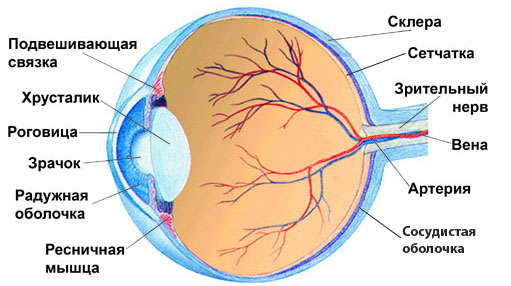
\includegraphics[width=0.95\columnwidth]{pictures/eye-scheme.jpg}
		\caption{}
		\label{fig:eye_scheme}
	\end{subfigure}%
	\begin{subfigure}{.5\textwidth}
		\centering
		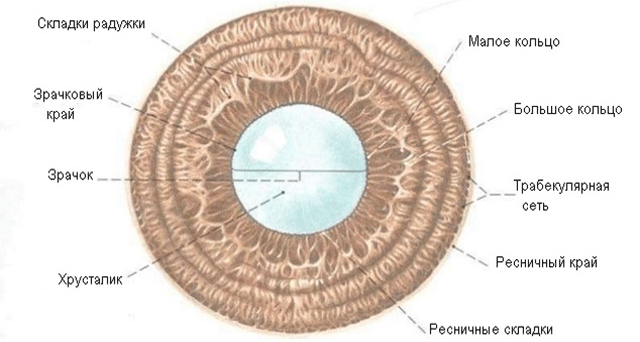
\includegraphics[width=0.95\columnwidth]{pictures/iris-structure.png}
		\caption{}
		\label{fig:iris_structure}
\end{subfigure}%
\caption{Строение глаза (а) и радужки (б)}
\label{fig:eye_and_iris_structure}
\end{figure}

На передней поверхности радужки выделяют зрачковый край (margo pupillaris) шириной 1 мм и ресничный край (margo ciliaris) шириной 3—4 мм. В области зрачкового края расположен сфинктер зрачка (sphincter pupillae) — мышца, суживающая зрачок; в области ресничного края находится дилататор зрачка (dilatator pupillae) — мышца, расширяющая зрачок (Рис.~\ref{fig:iris_structure}). Место соединения радужки с ресничным (цилиарным) телом называется корнем радужки, остальная её часть находится в свободном взвешенном состоянии в жидкости передней и задней камер глазного яблока~\cite{krasnov_1952}.

Структура радужки имеет вид губчатой ткани~\ref{fig:iris_structure_and_example}, состоящей из множества радиальных тонких перемычек (трабекул), образованных толстой адвентицией сосудов и окружающей их соединительной тканью. Между трабекулами располагаются углубления (лакуны и крипты). На границе зрачкового и ресничного края определяется зубчатая линия, или круг Краузе (малое кольцо радужки) — область прикрепления эмбриональной зрачковой сосудистой мембраны. Зрачок обрамлен темно-коричневой зрачковой каймой. На передней поверхности радужки видны складки, при узком зрачке более рельефно выделяются радиальные складки, при широком зрачке — концентрические~\cite{krasnov_1952}.

\begin{figure}[!h]
	\begin{subfigure}{.65\textwidth}
		\centering
		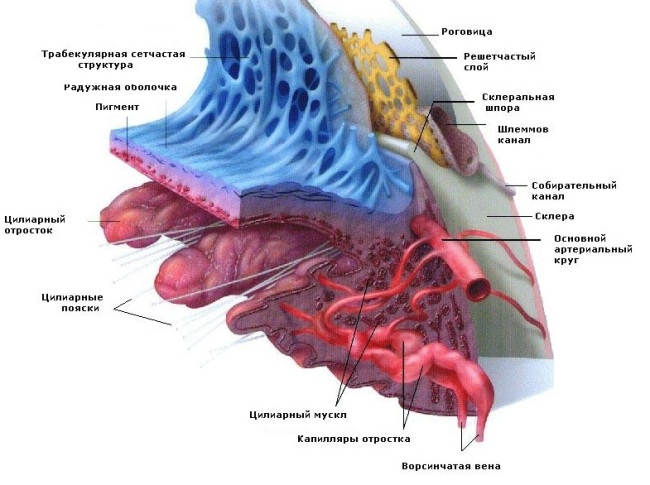
\includegraphics[width=0.95\columnwidth]{pictures/iris-trabelular-structure.jpg}
		\label{fig:iris_trabecular_structure}
	\end{subfigure}%
	\begin{subfigure}{.35\textwidth}
		\centering
		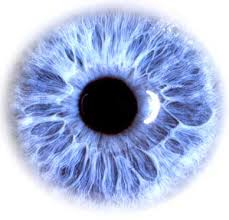
\includegraphics[width=0.95\columnwidth]{pictures/blue-iris-bagel.jpeg}
		\label{fig:blue_iris_bagel}
	\end{subfigure}%
	\caption{Структура радужки}
	\label{fig:iris_structure_and_example}
\end{figure}

Радужка имеет генетически обусловленные рисунок и цвет. Коричневый (темный) цвет наследуется по доминантному типу, голубой (светлый) — по рецессивному. Рисунок и цвет радужки слабо изменяются в течение жизни~\cite{arkhangelsky_1960}. Цвет радужки стабилизируется к 10—12 годам. В пожилом возрасте радужка становится несколько светлее вследствие дистрофических изменений. Также возможно появление пятен на поверхности радужки в связи с заболеваниями различных органов~\cite{krasnov_1952,arkhangelsky_1960}.

Сложность и особенности текстуры радужки делают её уникальным, высоко-информативным биометрическим признаком, который может быть использован в качестве идентификатора.


\section{Общая модель распознавания по радужке}
\label{sec:iris_recognition_basics}

Подавляющее большинство предложенных методов распознавания по радужной оболочке глаза используют следующую общую схему (Рис.~\ref{fig:irec_scheme_gen}):

\begin{figure}[!h]
	\centering
	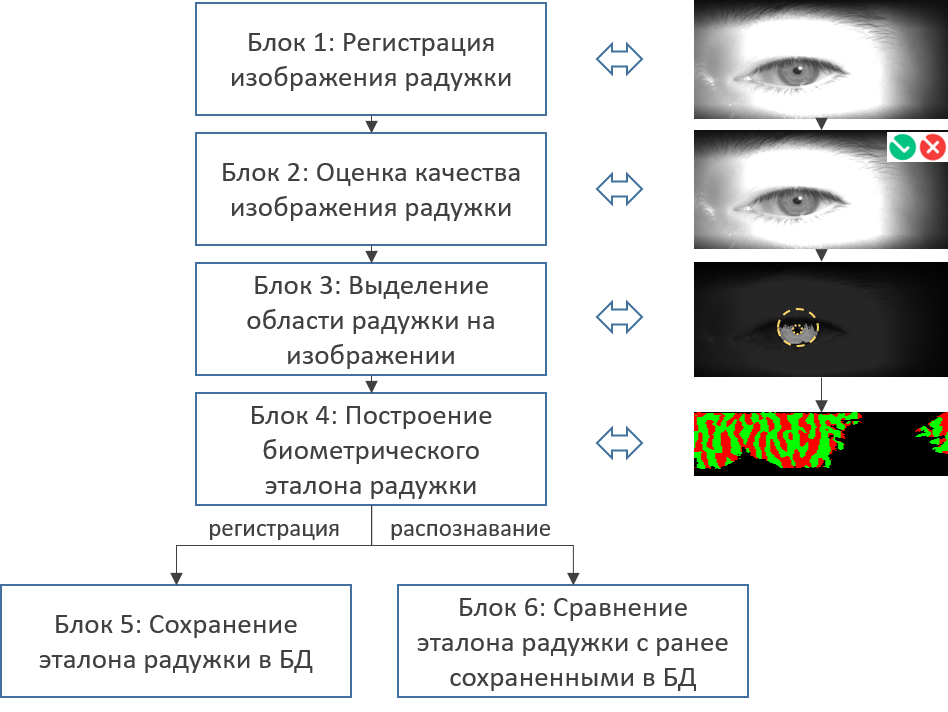
\includegraphics[width=0.75\columnwidth]{pictures/irec-scheme-gen.png}
	\caption{Общая схема распознавания по радужке}
	\label{fig:irec_scheme_gen}
\end{figure}

Регистрация изображения радужки (блок 1) осуществляется при помощи цифровой камеры в ближнем инфракрасном (БИК, 810-950 нм), либо в видимом (380-780 нм) диапазонах длин волн. При регистрации, как правило, так же используется активная диодная подсветка. Далее (блок 2) осуществляется оценка качества полученного изображения с точки зрения его пригодности для выделения радужки и формирования биометрического эталона. К блоку оценки качества часто относят подсистему защиты от подделки. Он может быть многостадийным и распределен между остальными блоками. Следующий за ним блок 3 осуществляет выделение радужки на изображении, т.е. отделение области изображения, относящейся к радужке, от фона и шума. В качестве шума здесь выступает множество элементов: веки, ресницы, блики и т.д. После того, как область радужки выделена, осуществляется построение биометрического эталона (блок 4).

\begin{figure}[!h]
	\centering
	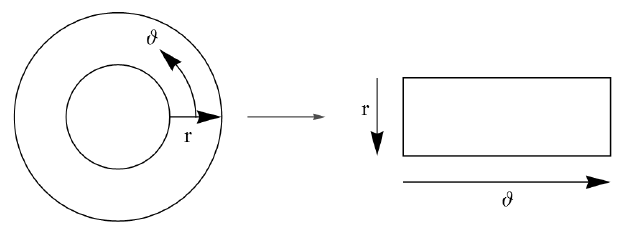
\includegraphics[width=0.5\columnwidth]{pictures/daugman-rubber-sheet.png}
	\caption{Преобразование изображения радужки}
	\label{fig:daugman_rubber_sheet}
\end{figure}

Данный этап часто включает преобразование изображения (Рис.~\ref{fig:daugman_rubber_sheet}), путем перехода из исходной Декартовой системы координат $(x,y)$ в полярную $(r,\theta)$~\eqref{eq:certesian-polar}, впервые предложенную в работе~\cite{daugman_1992}:
\begin{equation}\label{eq:certesian-polar}
	I(x(r, \theta), y(r, \theta)) \rightarrow I(r, \theta)
\end{equation}

\noindent
где $I(x,y)$ - исходное изображение радужки, $(x,y)$ координаты в Декартовой системе, а $(r,q)$ - соответствующие нормализованные координаты в полярной. $x(r,\theta)$ и $y(r,\theta)$ заданы в виде линейных комбинаций наборов точек границ зрачка $(x_p(\theta),y_p(\theta))$ и радужки $(x_i(\theta),y_i(\theta))$:
\begin{equation}\label{eq:certesian-polar2}
	\begin{split}
		x(r,\theta)=(1-r)\cdot x_p(\theta)+r\cdot x_i(\theta) \\
		y(r,\theta)=(1-r)\cdot y_p(\theta)+r\cdot y_i(\theta)
	\end{split}
\end{equation}

После того как биометрический шаблон радужки построен, в зависимости от текущего сценария (регистрация/распознавание) он либо сохраняется в БД (блок 5), либо сравнивается с эталонами, сохраненными в БД ранее (блок 6). При построении шаблона также часто используется процедура выбора наилучшего (-их) по заранее заданным критериям, что позволяет снизить ошибки распознавания.

\section{Особенности мобильной биометрии радужки}
\label{sec:mobile_iris_features}

Значительная доля платежных транзакций осуществляется посредством мобильных платежных систем, и эта доля стремительно растет~\cite{wpr_2017}. При работе с Samsung Pay, Apply Pay и Android Pay пользователю предлагается использовать один из возможных способов аутентификации, среди которых уже сейчас присутствует биометрический шаблон отпечатков пальцев (Рис.~\ref{fig:mobile_payment_pics}).

\begin{figure}[!h]
	\centering
	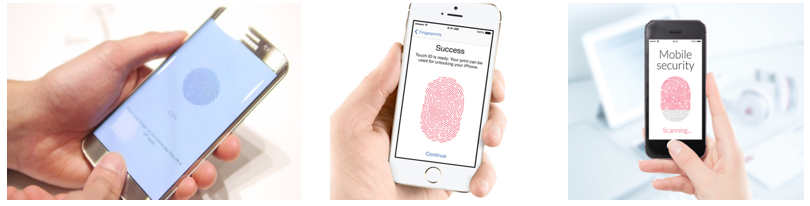
\includegraphics[width=0.95\columnwidth]{pictures/mobile_payment_pics.png}
	\caption{Использование отпечатков пальцев при совершении платежной транзакции с мобильного устройства}
	\label{fig:mobile_payment_pics}
\end{figure}


Как было упомянуто ранее, технология распознавания по радужке обладает рядом преимуществ по сравнению с распознаванием по иным биометрическим признакам, в том числе отпечаткам пальцев. Структура радужки является устойчивым, хорошо выраженным и высоко-информативным биометрическим признаком, практически не подвергающимся изменениям в течение жизни. Кроме этого, процедура распознавания по радужке является бесконтактной. Перечисленные свойства позволяют обеспечить удобство использования, более высокую точность распознавания и надежность биометрических систем идентификации, построенных на основе данного биометрического признака и, как следствие, расширение рынка мобильных устройств.

В качестве информации, используемой для построения биометрического шаблона в системах биометрической идентификации личности по радужной оболочке глаза, выступает изображение радужки.

Работа с мобильным устройством накладывает дополнительные ограничения на применения биометрической системы распознавания по радужке и, как следствие, к ней выдвигаются дополнительные требования. Система должна обеспечивать работу в условиях постоянно изменяющихся внешних условий среды. Распознавание должно производиться в помещении, на улице, в солнечную и пасмурную погоду, учитывать возможность ношения очков, контактных линз и др. Система должна обеспечивать удобство использования, т.е. учитывать поведение пользователя, возможные моргания, тряску рук, направление взгляда и так далее. Система должна обеспечивать возможность работы в реальном времени на мобильном устройстве с ограниченным количеством потребляемой памяти и вычислительных ресурсов, обеспечивая при этом высокую точность распознавания.

\begin{figure}[!h]
	\centering
	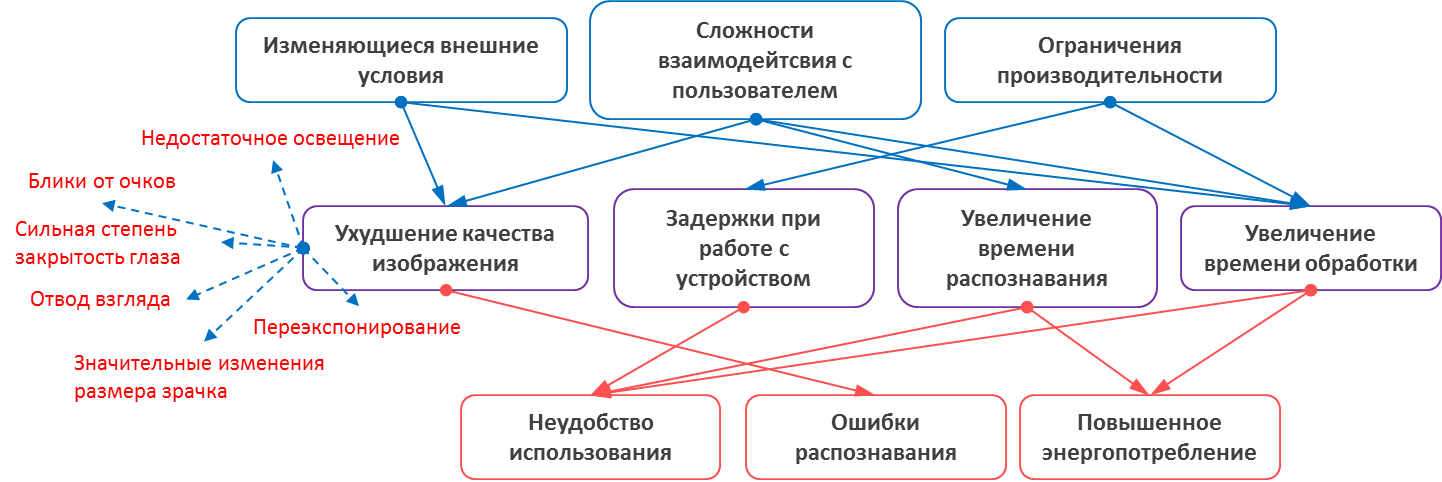
\includegraphics[width=0.95\columnwidth]{pictures/iris_mobile_problems.png}
	\caption{Основные проблемы при распознавании по радужке с мобильного устройства}
	\label{fig:iris_mobile_problems}
\end{figure}

Неучёт вышеперечисленных требований приводит к ухудшению качества изображения (Рис.~\ref{fig:iris_mobile_problems},~\ref{fig:iris_iamge_quality_degradation})~\cite{dorairaj_perf_eval}, а в некоторых случаях даже к невозможности его получения.

\begin{figure*}[!h]
	\begin{subfigure}{.33\textwidth}
		\centering
		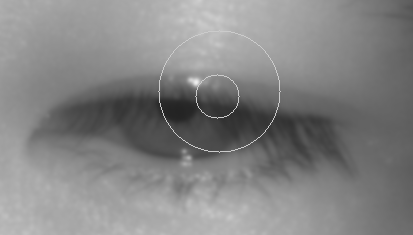
\includegraphics[width=0.95\columnwidth,height=3.5cm]{pictures/gaze-away-occlusion.png}
		\caption{}
		\label{fig:gaze_away_occlusion}
	\end{subfigure}%
	\begin{subfigure}{.33\textwidth}
		\centering
		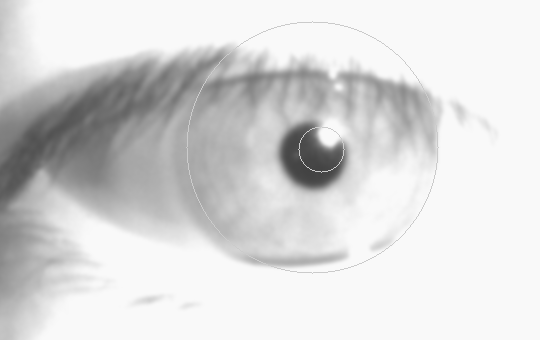
\includegraphics[width=0.95\columnwidth,height=3.5cm]{pictures/over-exposure.png}
		\caption{}
		\label{fig:over_exposure}
	\end{subfigure}%
	\begin{subfigure}{.33\textwidth}
		\centering
		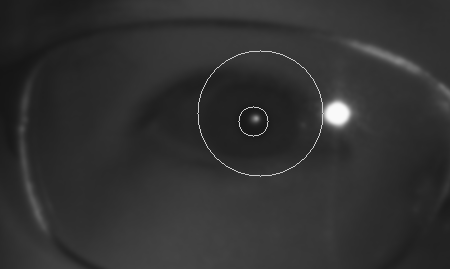
\includegraphics[width=0.95\columnwidth,height=3.5cm]{pictures/poor-contrast.png}
		\caption{}
		\label{fig:poor_contrast}
	\end{subfigure}%
	\caption{Ухудшение качества изображения при распознавании по радужке с мобильного устройства, влекущее за собой ошибки сегментации радужки: а) отвод взгляда, перекрытие веками, б) пере-экспонирование, в) низкий контраст, блик от очков}
	\label{fig:iris_iamge_quality_degradation}
\end{figure*}

Ухудшение качества изображения приводит к снижению точности распознавания, что ставит под сомнение возможность применения таких биометрических систем при осуществлении различного рода транзакций (Рис.~\ref{fig:iris_mobile_problems}).

\section{Выводы к первой главе}

Произведен обзор биометрических методов распознавания человека. Приведено сравнение различных биометрических характеристик человека с точки зрения их универсальности, уникальности, стабильности и собираемости. Рассмотрены основные области применения и направления развития биометрических методов. Описаны структура и свойства радужной оболочки глаза. Показаны её преимущества и недостатки как уникальной БХЧ. Приведена общая схема распознавания по радужке от процедуры регистрации изображения до вычисления степени схожести и принятия решения об идентичности/неидентичности двух радужек. Рассмотрены особенности использования радужки в качестве БХЧ при распознавании человека с мобильного устройства.